\toftagthis{krestan}
\song{Panenka}{Robert Křesťan}{70pt}{1}{
\verse{1}Co \D{}skrýváš za \G{}víčky a \D{}plameny \G{}svíčky,\\
snad \D{}houf bílých holubic nebo jen \A{}žal?\\
Tak \G{}odplul ten \D{}prvý den, \G{}zmáčený \D{}krví,\\
ani pouťovou panenku \A[7]{}nezane\D{}chal.

\chorus{}Otevři \G{}oči, ty \D{}uspěcha\A{}ná,\\
\G{}dámo \D{}uplaka\A{}ná,\\
\G{}otevři \D{}oči, ta \G{}hloupá noc \D{}končí,\\
a mír je \A[7]{}mezi ná\D{}ma.

\verse{2}Už si oblékni šaty i řetízek zlatý\\
a umyj se, půjdeme na karneval.\\
A na bílou kůži ti napíšu tuší,\\
že dámou jsi byla a zůstáváš dál.\\
\textbf{R:}\\
}


\toftagthis{anglicke}
\song{Perfect Day}{Lou Reed}{40pt}{1}{
\E{} \hskip 1em \Am{} \hskip 2em \E{} \hskip 1em \Am{}\\
\verse{1}\Am{}Just a \D{}perfect day,\G{} drink sangria \C{}in the park,\\
\F{}then later when \Dm{}it gets dark we go\E{} home.

\verse{2}Just a perfect day, feed animals in the zoo,\\
then later a movie, too, and then home.

\chorus{}Oh, \A{}it's such a \D{}perfect day,\\
\Csm{}I'm glad I spent it with \D{}you.\\
\A{}Oh, such a \E{}perfect day,\\
\revrpt{} you just \Fsm{}keep me \E{}hanging \D{}on, \rpt{}

\verse{3}Just a perfect day, problems all left alone,\\
weekenders on our own, it's such fun.

\verse{4}Just a perfect day, you made me forget myself,\\
I thought I was someone else, someone good.\\
\textbf{R:}

\revrpt{} \Csm{}You're gonna \G{}reap just what you \D{}sow.\A{} \hskip 1em \rpt{}\\
}


\toftagthis{nohavica}
\song{Petěrburg}{Jaromír Nohavica}{12pt}{0.92}{
\textls[-20]{\verse{1}\Am{}Když se snáší noc na střechy Petěrburgu, \F{}padá \E{}na mě \Am{}žal,\\
\textls[-35]{zatoulaný pes nevzal si ani kůrku \F{}chleba, kterou \E{}jsem mu \Am{}dal.}

\chorus{}\revrpt{} \C{}Lásku moji \Dm{}kníže I\E{}gor si bere,\\
\F{}nad sklenkou \Ds[dim]{}vodky \hskip 0.5em \H[7]{}hraju si \E{}s revolverem,\\
\Am{}havran usedá na střechy Petěrburgu, \F{}čert a\E{}by to \Am{}spral. \rpt{}

\textsl{Mezihra (akordy sloka + 2$\times$ ref.)} 

\verse{2}Nad obzorem letí ptáci slepí v záři červánků,\\
moje duše, široširá stepi, máš na kahánku.

\chorus{}\revrpt{} Mému žalu na světě není rovno,\\
vy jste tím vinna, Naděždo Ivanovno,\\
vy jste tím vinna, až mě zítra najdou s dírou ve spánku. \rpt{}\\}
\noexport{
~\\
\hskip -17pt \textbf{\large Mezihra:}
\vskip -2pt

\begin{figure}[h]
\leftskip -5pt
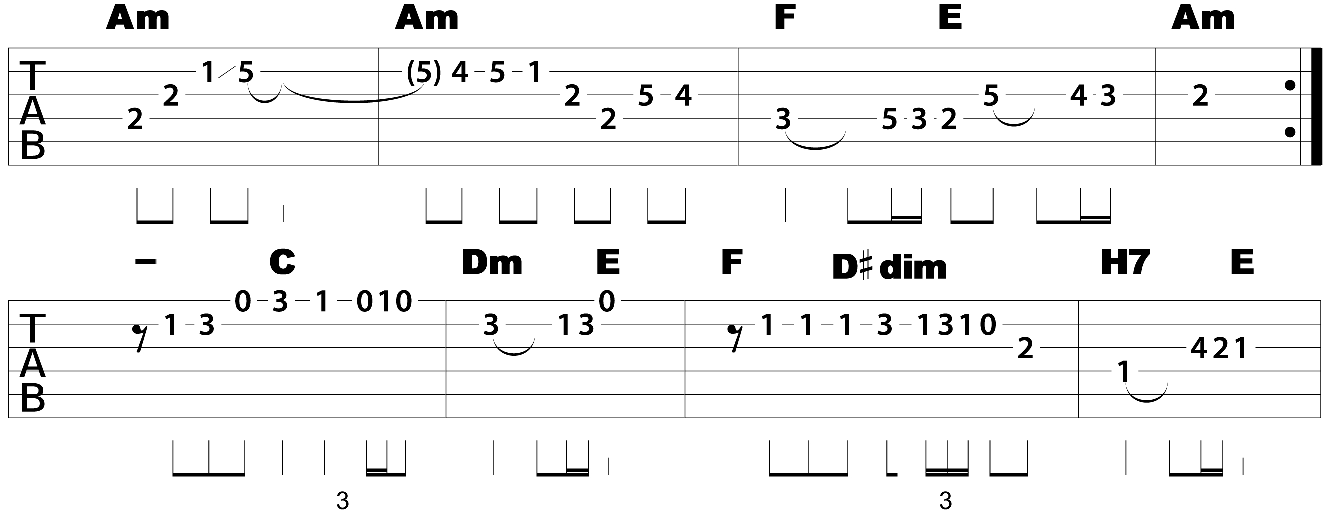
\includegraphics[width=370pt, height=133pt]{res/peterburg.pdf}
\vskip -15pt
\end{figure}
}
}

\toftagthis{nohavica}
\song{Pijte vodu}{Jaromír Nohavica}{65pt}{0.88}{
\chorus{}\revrpt{} \C{}Pijte vodu, pijte pitnou vodu,\\
pijte vodu a \G[7]{}nepijte \C{}rum. \rpt{}

\vskip -1ex
\verse{1}Jeden smutný ajznboňák\\
pil na pátém nástupišti Air Cognac.\\
Huba se mu slepila,\\
diesel lokomotiva ho zabila.\\
\textbf{R:}

\vskip -1.5ex
\verse{2} V rodině u Becherů\\
pijou becherovku přímo ze džberů.\\
Proto všichni Becheři\\
mají trable s játrama a páteří.\\
\textbf{R:}

\vskip -1.5ex
\verse{3}Pil som vodku značky Gorbatschow\\
a potom povedal som všeličo a volačo.\\
Vyfásol som za to tri roky,\\
teraz pijem chlorované patoky.\\
\textbf{R:}

\vskip -1.5ex
\verse{4}Jesteśmy chłopci z Warszawy,\\
jeżdżimy pociągiem za robotą do Ostrawy.\\
Cztery litry wódki a mnóstwo piw,\\
po prostu bardzo fajny kolektyw.\\
\textbf{R:}

\vskip -1.5ex
\verse{5}Jedna paní v Americe\\
ztrapnila se převelice.\\
Vypila na ex rum\\
a poblila jim Bílý dům.\\
\textbf{R:}\\
}


\toftagthis{sverakuhlir}
\song{Píseň proti trudomyslnosti}{J. Uhlíř / Z. Svěrák}{13pt}{1}{
\textls[-10]{\D{}Polární noc má zvláštní moc, každého přepadne smu\A[7]{}tek,\\
Němec i Brit, křesťan i Žid, každý by nejradši ute\D{}k',\\
ba i ti \G{}šikovní Žapon\D{}ci se sila\E[7]{}mi jsou na kon\A[7]{}ci,\\
jen jeden z \D{}národů nesko\G{}ná, hrůzy seve\D{}ru slavně \A[7]{}překo\D{}ná!\\}
~\\
Tam, kde hy-, tam, kde hy-, tam, kde hynou vl\A[7]{}ci,\\
tam, kde hy-, tam, kde hy-, tam kde hynou vl\D{}ci,\\
tam, kde hy-, tam, kde hy-, tam kde hynou so\G{}bi,\\
\A[7]{}Čech se přizpůso\D{}bí! \A[7]{}Čech se přizpůso\D{}bí!\A[7]{}\hskip 1.8em \D{}\\
}


\toftagthis{slovenske}
\song{Po schodoch}{Richard Müller}{35pt}{1}{
\verse{1}\Am{}Výťah opäť nechodí, tak \G{}zdolať 13 poschodí\\
\F{}zostáva mi \G{}znova po svo\Am{}jich.\\
Na schodoch čosi šramotí a neón kde tu nesvieti,\\
ešte že sa po tme nebojím.

\verse{2}Počuť hlasné stereo aj výstrahy pred neverou\\
ktosi čosi vŕta v paneloch.\\
Tatramatky ródeo zas mieša sa tu s operou,\\
\F{}všetko počuť \G{}cestou po scho\Am{}doch.\Em{}

\chorus{}\revrpt{} Cestou \Am{}po schodoch, \Em{}po schodoch,\\
\F{}poznávam \G{}poschodia,\\
poznám \Am{}po schodoch, \Em{}po zvukoch,\\
\F{}čo sme kto \Em{}za ľu\Am{}dia. \rpt{}

\verse{3}Štekot smutnej kólie, za premárnené prémie\\
vyhráža sa manžel rozvodom.\\
Disko, tenis, árie, kritika televízie,\\
oddnes chodím iba po schodoch.\\
\textbf{R:}
}


\toftagthis{nedvedi}
\song{Podvod}{Jan Nedvěd}{15pt}{0.9}{
\capo{2}
\verse{1}\Em{}Na dlani jednou z tvých řas, do tmy se \Am{}koukám,\\
\D{}hraju si písničky tvý, co sem ti \G{}psal.\\
Je skoro \Am{}půlnoc a z kostela \Am[/C]{}zvon mi noc připo\Em{}míná,\\
půjdu se \Am{}mejt a pozhasí\Am[/C]{}nám, co bude \H[7]{}dál?

\verse{2}Pod polštář dopisů pár, co poslalas dávám,\\
píšeš, že ráda mě máš a trápí tě stesk.\\
Je skoro půlnoc a z kostela zvon mi noc připomíná,\\
půjdu se mejt a pozhasínám, co bude dál?

\chorus{}Chtěl jsem to \Am{}ráno, kdy naposled snídal jsem s tebou,\\
ti \Em{}říct, že už ti nezavolám,\\
pro jednou pitomou \Am{}holku, pro pár noci \D{}touhy,\\
podved' jsem \G{}všechno, o čem doma si \H[7]{}sníš,\\
teď je mi to \Em{}líto.

\verse{3}Kolikrát člověk může mít rád tak opravdu z lásky,\\
dvakrát či třikrát -- to ne, i jednou je dost.\\
Je skoro půlnoc a z kostela zvon mi noc připomíná,\\
půjdu se mejt a pozhasínám, co bude dál?\\
\textbf{R: ($2\times$)}
}


\toftagthis{kabat}
\song{Pohoda}{Kabát}{80pt}{1}{
\vskip 8pt
\CHORD{\revrpt{}}{} \hskip 0.7em \D{} \hskip 1em \A{} \hskip 1em \E{} \hskip 1em \Hm{} \hskip 2em \CHORD{\rpt}{}\\
\verse{1}\Fsm{} Vezmu tě, má milá, \Csm{}rovnou k nám,\\
\Fsm{} kolem louky, lesy, \Csm{}hejna vran,\\
\Fsm{} všude samá \E{}kráva, samej \Hm{}vůl.

\verse{2}Máme kino, máme hospodu,\\
v obci všeobecnou pohodu,\\
máme hujer, žito, chléb i sůl.

\chorus{}\D{}Když se u nás chlapi \A{}poperou,\\
tak jenom \E{}nožem anebo \Hm{}sekerou,\\
v zimě tam \D{}dlouhý noci \A{}jsou\\
a tuhej \Hm{}mráz.\Hm{}\\
Jak jsou naše cesty zavátý,\\
tak vezmem vidle anebo lopaty,\\
když něco nejde, co na tom sejde,\\
my máme čas.

\verse{3}Chlapi někdy trochu prudký jsou,\\
holky s motykama tancujou,\\
s ranní rosou táhnou do polí.

\clearpage
\verse{4} Nikdo se tam nikam nežene,\\
máme traktory a ne, že ne,\\
až to spatříš, ledy povolí.\\
\textbf{R:}

\verse{5}Hoří les a hoří rodnej dům,\\
hoří velkostatek sousedům,\\
to je smůla, drahá, podívej.

\verse{6}Hasiči to stejně přejedou,\\
oni si moc dobře nevedou,\\
schovej sirky, ať je neviděj.\\
\textbf{R: ($2\times$)}
}


\toftagthis{nohavica}
\song{Pochod marodů}{Jaromír Nohavica}{30pt}{1}{
\verse{1}\Dm{}Krabička cigaret a \F{}do kafe \C{}rum, \Bb{}rum, \Dm{}rum,\\
dvě vodky a fernet a teď, \F{}doktore, \C{}čum, \Bb{}čum, \Dm{}čum,\\
chra\Gm{}pot v hrud\Bb{}ním ko\Dm{}ši, no \Gm{}to je \Bb{}záži\A{}tek,\\
\Dm{}my jsme kámoši řidi\F{}čů sani\C{}tek, -\Bb{}tek, -\Dm{}tek.

\verse{2}Měli jsme ledviny, ale už jsou nadranc, -dranc, -dranc,\\
i tělní dutiny už ztratily glanc, glanc, glanc,\\
u srdce divný zvuk, co je to, nemám šajn,\\
je to vlastně fuk, žijem fajn, žijem fajn, fajn, fajn.

\chorus{}\Dm{}Cirhóza, \F{}trombóza, \C{}dávivý \F{}kašel,\\
\Gm{}tuberku\Dm{}lóza -- \A{}jó, to je \Dm{}naše!\\
Neuróza, \F{}skleróza, \C{}ohnutá \F{}záda,\\
\Gm{}paraden\Dm{}tóza, no \A{}to je pa\Dm{}ráda!\\
Jsme \Gm{}slabí na tě\Dm{}le, ale \C{}silní na du\F{}chu,\\
\Gm{}žijem vese\Dm{}le, \hskip 1em \A{}juchuchuchu\Dm{}chu!

\verse{3}Už kolem nás chodí pepka mrtvice, -ce, -ce,\\
tak pozor, marodi, je zlá velice, -ce, -ce,\\
zná naše adresy a je to čiperka,\\
koho chce, najde si, ten natáhne perka, -rka, -rka.

%\leftskip 50pt
\verse{4}Zítra nás odvezou, bude veselo, -lo, -lo,\\
doktoři vylezou na naše tělo, -lo, -lo,\\
budou nám řezati ty naše vnitřnosti\\
a přitom zpívati ze samé radosti, -sti, -sti.

\chorus{}Zpívati: \Dm{}Cirhóza, \F{}trombóza, \C{}dávivý \F{}kašel,\\
\Gm{}tuberku\Dm{}lóza, hele, \A{}já jsem to \Dm{}našel!\\
Neuróza, \F{}skleróza, \C{}křivičná \F{}záda,\\
\Gm{}paraden\Dm{}tóza, no \A{}to je pa\Dm{}ráda!\\
Byli \Gm{}slabí na tě\Dm{}le, ale \C{}silní na du\F{}chu,\\
\Gm{}žili vese\Dm{}le, než \A{}měli poru\D{}chu!\\
}


\toftagthis{nohavica}
\song{Potulní kejklíři}{Jaromír Nohavica}{40pt}{0.8}{
\verse{1}\Am{} Potulní kejklíři \Em{}jdou zasněženou plá\Am{}ní, \hskip 1em \Em{}\\
\Am{} v obitém talíři \Em{}vaří vítr ke snída\Am{}ni. \hskip 1em \Em{}\\
\C{} S cvičenou opičkou \G{}na rameni,\\
\Am{}životem\Dm{} malin\G{}ko \C{}unave\E[7]{}ni,\\
\Am{}potulní kejklíři \Em{}jdou bílou plá\Am{}ní. \hskip 1em \Em{}

\verse{2}V kovárně na kraji vsi všechen sníh už ztál,\\
dobrý kovář odžene psy a pozve je dál,\\
sláma je postelí i peřinou\\
a oni jeden k druhému se přivinou\\
a zítra na návsi začíná candrbál.

\chorus{}\revrpt{} \Am{}Kejklíři, \Em{}kejklíři \Am{}jdou\ldots{}\Em{} \hskip 1.5em \rpt{} 

\verse{3}Po schodech kostela poskakuje míč,\\
muž s tváří anděla ohýbá železnou tyč.\\
A krásná dívka jménem Marína\\
zatančí tanec pohanského bůžka Odina\\
a zítra po polednách budou zase pryč.\\
\textbf{R:}

\verse{4}Vozíček z lipových dřev po hlíně drkotá,\\
červená nepokojná krev je erbem života,\\
všechno, co chceme, leží před námi\\
za devatero poli, devatero řekami,\\
nad zimní krajinou slunce blikotá.\\
\textbf{R: $(2\times)$}\\
}


\toftagthis{folk}
\song{Pověste ho vejš}{Michal Tučný}{45pt}{0.9}{
\rec{\emph{\Em{}}Na dnešek jsem měl divnej sen,\\
slunce pálilo a před salonem\\
stál v prachu dav, v tvářích cejch očekávání,\\
uprostřed šibenice z hrubých klád.\\
Šerifův pomocník sejmul z hlavy odsouzenci kápi\\
a dav zašuměl překvapením.\\
I já jsem zašuměl překvapením.\\
Ten odsouzenec jsem byl já\\
a šerif četl neúprosným hlasem rozsudek:}

\chorus{}Pověste ho \Em{}vejš, ať se houpá,\\
pověste ho \G{}vejš, ať má \D{}dost.\\
Pověste ho \Am{}vejš, ať se \Em{}houpá,\\
že tu \D{}byl nezvanej \Em{}host.

\verse{1} Pověste ho, že byl jinej,\\
že tu s náma dejchal stejnej vzduch.\\
Pověste ho, že byl línej\\
a tak trochu dobrodruh.

\verse{2}Pověste ho za El Passo,\\
za snídani v trávě a lodní zvon.\\
Za to, že neoplýval krásou,\\
že měl \C{}country rád a že se \H[7]{}uměl smát i \Em{}vám.

\verse{*}Nad hla\G{}vou mi slunce \D{}pálí,\\
konec \Am{}můj nic neod\G{}dá\D{}lí.\\
Do svých \G{}snů se dívám \D{}zdáli,\\
a \Am{}do uší mi stále zní tahle \H[7]{}moje píseň poslední.

\verse{3} Pověste ho za tu banku,\\
v který zruinoval svůj vklad.\\
Za to, že nikdy nevydržel\\
na jednom místě stát.

\verse{*} Nad hlavou\ldots{}\\
\textbf{R:}

\verse{4} Pověste ho za tu jistou,\\
který nesplnil svůj slib,\\
že byl zarputilým optimistou\\
a tak dělal spoustu chyb.

\verse{5} Pověste ho, že se koukal,\\
že hodně jed' a hodně pil,\\
že dal přednost jarním loukám\\
a pak se \C{}oženil a pak se \H[7]{}usadil a \Em{}žil.\\
\textbf{R: $(2\times)$}
}

\toftagthis{suchyslitr}
\song{Pramínek vlasů}{Jiří Suchý}{50pt}{0.95}{
\verse{1}Když měsíc \C{}rozlije\Am{} světlo své \F[6]{}po kraji\G[6]{}\\
a hvězdy řeknou, že čas je jít spát,\\
pramínek vlasů jí ustřihnu potají,\\
komu --  no \C{}přece té,\F[7]{} kterou mám \C{}rád.\G[7]{}

\verse{2}Pramínek vlasů jí ustřihnu potají,\\
já blázen pod polštář chci si ho dát.\\
Ačkoliv sny se mi zásadně nezdají,\\
věřím, že dnes v noci budou se zdát.

\chorus{}O sny mě \Bb{}připraví teprve \C{}svítání,\\
zpěv ptáků v \Bb{}oblacích a modré \C{}nebe.\\
Od vlasů, \F{}jichž jsem se dotýkal \C{}ve spaní,\\
nový den \Ab[7]{}nůžkama odstřihne \G{}tebe.

\verse{3}A na bílém polštáři, do kroužku stočený,\\
zbude tu po tobě pramínek vlasů.\\
Já nebudu vstávat, dál chci ležet zasněný,\\
je totiž neděle a mám dost času.\\
\textbf{R:}

\verse{4}A na bílém polštáři\dots\\
\revrpt{}\ldots{}je totiž neděle a mám dost času. \rpt{}\\
}



\toftagthis{ceskekapely}
\song{Proklínám}{Janek Ledecký}{20pt}{1}{
\verse{1}
Prázdnej \Am{}byt je jako \F{}past, 
kde \Dm{}růže uvad\C{}nou. \G{}\\
\Am{}Potisící\F{} čtu tvůj dopis \Dm{}na rozlouče\G{}nou.\\\
\C{}Píšeš že \Am{}odcházíš, když \F{}den se s nocí \C{}stří\G{}dá.\\
\Am{}Vodu z vína\F{} udělá, kdo \Dm{}dobře nehlí\G{}dá. Píšeš:

\chorus{}\C{}Proklíná\G{}m,\hskip 0.3em \Am{} ty tvoje \F{}ústa, proklíná\C{}m\\
tvoje \G{}oči ledo\Am{}vý,
v \F{}srdci jen sníh,\C{} sám a sá\G{}m.\\
\Am{}Ať nikdy \F{}úsvit nespatř\C{}íš,
na ústa mř\G{}íž,  oči oslep\Am{}nou.\\
Ať \F{}do smrti seš s\C{}ám.

\verse{2}Tvoje oči jsou jak stín a tvář -- den, když se stmívá.\\
Stromy rostou čím dál výš a pak je čeká pád.\\
Sám s hlavou skloněnou,všechny lásky budou zdání.\\
Potisící čtu tvůj dopis na rozloučenou. Píšeš:\\
\textbf{R:} \dots ať \F{}do smrti seš s\C{}ám a sá\G{}m.\\
Ať nikdy úsvit nespatříš\dots\\
}


\toftagthis{cechomor}
\song{Proměny}{Čechomor}{50pt}{1}{
\verse{1}\Am{}Darmo sa ty trápíš, \G{}můj milý sy\C{}nečku,\\
nenosím já tebe, \E[7]{}nenosím v sr\Am{}déčku,\\
přece tvo\G{}ja \C{}ne - \G{}bu - \C{}du, \Dm{}ani jednu \E{}hodi\Am{}nu.

\verse{2}Copak sobě myslíš, má milá panenko,\\
vždyť ty jsi to moje rozmilé srdénko\\
a ty musíš býti má, lebo mi tě Pán Bůh dá.

\verse{3}A já sa udělám malú veveričkú\\
a já ti uskočím z dubu na jedličku,\\
přece tvoja nebudu, ani jednu hodinu.

\verse{4}A já chovám doma takú sekérečku,\\
ona mi podetne dúbek i jedličku\\
a ty musíš býti má, lebo mi tě Pán Bůh dá.

\verse{5}A já sa udělám tú malú rybičkú\\
a já ti uplynu preč po Dunajíčku,\\
přece tvoja nebudu, ani jednu hodinu.

\verse{6}A já chovám doma takovú udičku,\\
co na ni ulovím kdejakú rybičku\\
a ty přece budeš má, lebo mi tě Pán Bůh dá.

\optVerse{-30pt}{20pt}{-15pt}{
\emph{housle}\ \ \revrpt{} \textbf{\sffamily Ami \ Ami \ F \ C \ F \ C \ G \ G} \rpt
}

\verse{7}A já sa udělám tú velikú vranú\\
a já ti uletím na Uherskú stranu,\\
přece tvoja nebudu, ani jednu hodinu.

\verse{8}A já chovám doma starodávnú kušu,\\
co ona vystřelí všeckým vranám dušu\\
a ty musíš býti má, lebo mi tě Pán Bůh dá.

\verse{9}A já sa udělám hvězdičkú na nebi\\
a já budu lidem svítiti na nebi,\\
přece tvoja nebudu, ani jednu hodinu.

\hskip -8pt\verse{10}A sú u nás doma takoví hvězdáři,\\
co vypočítajú hvězdičky na nebi\\
\revrpt{} a ty musíš býti má, lebo mi tě Pán Bůh dá. \rpt{}

\optVerse{-30pt}{20pt}{-15pt}{
\emph{housle}\ \ \revrpt{} \textbf{\sffamily Ami \ Ami \ F \ C \ F \ C \ G \ G} \rpt
}
}


\toftagthis{chinaski}
\song{První signální}{Chinaski}{35pt}{1}{
\verse{1}Až si \G{}zejtra ráno \C{}řeknu zase \Em{}jednou provždy dost,\\
\G{}právem se mi \C{}budeš tiše \Em{}smát.\\
Jak omluvit si svoji slabost, nenávist a zlost,\\
když za všechno si můžu vlastně sám.

\chorus{}Za \Am{}spoustu dní, možná za \C{}spoustu let,\\
až se mi \G{}rozední, budu ti \D{}vyprávět\\
na první signální, jak jsem vobletěl svět,\\
jak tě to vomámí a nepustí zpět.\\
Jaký si to \F{}uděláš, \Bb{}takový to \Dm{}máš.\\
Jaký si to \F{}uděláš, \Bb{}takový to \Dm{}máš.

\verse{2}Až se dneska večer budu tvářit zas jak Karel Gott,\\
budu zpívat vampam tydam pam.\\
Všechna sláva, polní tráva, ale peníz přijde vhod,\\
jak jsem si to udělal, tak to mám.

\chorus{}Za spoustu dní \dots{}\\
\dots jak tě to vomámí a nepustí zpět.\\
Ná nana \Am{}ná naná, ná nana \C{}ná naná \dots

\revrpt{} Jaký si to uděláš, takový to máš. \rpt{}\\
}


\toftagthis{nohavica}
\song{Přítel}{Jaromír Nohavica}{30pt}{0.9}{
\vskip -5pt
\capo{2}
\crdheight=2.2ex
\verse{1}Jestlipak \G{}vzpomínáš si ještě na ten \D[/F$\sharp$]{}čas,\\
táhlo nám \Am[7/E]{}na dvacet a slunko bylo v \D{}nás,\\
\Am{}vrabci nám jedli z ruky, \C{}život šel bez záruky,\\
\G{} ale taky bez pří\D[/F$\sharp$]{}kras.

\verse{2}Možná, že hloupý, ale krásný byl náš svět,\\
zdál se nám opojný jak dvacka cigaret\\
a všechna tajná přání plnila se na počkání\\
anebo rovnou hned.

\chorus{}\Am{}Kam jsme se poděli, \C{}kam jsme se to poděli,\\
\G{}kde je ti \D[/F$\sharp$]{}konec, m\Em[7]{}ůj jediný příteli,\\
\Am{}zmizels mi, nevím \D{}kam,\\
\C[add9]{}sám, sám, sám, jsem tady \G{}sám.\D[/F$\sharp$]{} \hskip 2.5em \Am[7/E]{} \hskip 3.7em \D{}

\verse{3}Jestlipak vzpomínáš si ještě na tu noc,\\
jich bylo pět a tys mi přišel na pomoc,\\
jó, tehdy nebýt tebe, tak z mých dvanácti žeber\\
nezůstalo příliš moc.

\verse{4}Dneska už nevím, jestli přiběh' by jsi zas,\\
jak tě tak slyším, máš už trochu vyšší hlas,\\
a vlasy, vlasy kratší, jó, bývali jsme mladší,\\
no a co, vem to ďas.

\chorus{}Kam jsme se poděli, kam jsme se to poděli,\\
kde je ti konec, můj jediný příteli,\\
zmizels mi, nevím kam,\\
sám, sám, sám, peru se teď sám.

\verse{5}Jestlipak vzpomínáš si ještě na ten rok,\\
každá naše píseň měla nejmíň třicet slok\\
a my dva jako jeden ze starých reprobeden\\
přes moře jak přes potok.

\verse{6}Tvůj děda říkal: \uv{Ono se to uklidní,}\\
měl pravdu, přišla potom spousta malých dní\\
a byla velká voda, vzala nám, co jí kdo dal,\\
a tobě i to poslední.

\chorus{}Kam jsme se poděli, kam jsme se to poděli,\\
kde je ti konec, můj jediný příteli,\\
zmizels mi, nevím kam,\\
sám, sám, sám, zpívám tady sám.

\verse{7}Jestlipak vzpomínáš si na to, jakýs byl,\\
jenom mi netvrď, že tě život naučil,\\
člověk, to není páčka, kterou si, kdo chce, mačká,\\
to už jsem dávno pochopil.

\verse{8}A taky vím, že srdce rukou nechytím,\\
jak jsem se změnil já, tak změnil ses i ty,\\
a přesto líto je mi, že už nám nad písněmi\\
společný slunko nesvítí.

\chorus{}Kam jsme se poděli, kam jsme se to poděli,\\
kde je ti konec, můj bývalý příteli,\\
zmizels mi, nevím kam,\\
sám, sám, sám, dýchám tady sám.\\
}
